

\section{Theoretical analysis for pPCA}
\label{sec:lin_VAE_analysis}
We aim to understand the theoretical advantages and disadvantages of each objective function used for training VAEs and how they impact downstream decision-making procedures.
Because intractability prevents us from deriving sharp constants in general models, to support a precise theoretical analysis, we consider probabilistic principal component analysis (pPCA)~\cite{tipping1999probabilistic}. pPCA is a linear model for which posterior inference is tractable. 
Though the analysis is a special case, we believe that it provides an intuition for performance of our decision-making procedures more generally because, for many of the models that are used in practice, a Gaussian distribution approximates the posterior well, as demonstrated by the success of the Laplace approximation~\cite{laplace1986}.

In pPCA, the latent variables $z$ generate data $x$. We use an isotropic Gaussian prior on $z$ and a linear model with spherical Gaussian observation model for $x$:
\begin{align}
\label{eq:lin_vae_gen}
\begin{split}
p_\theta(z) &=\textrm{Normal}(0, I) \\
p_\theta(x \mid z) &= \textrm{Normal}(Wz + \mu, \sigma^2I).
\end{split}
\end{align}
To make model selection challenging, we follow~\cite{Turner2011} and parameterize $\sigma^2 = \nicefrac{1}{(1 - \lambda^2)}$ as well as $W_{ij} = e^\lambda W'_{ij}$ if $i \neq j$ and $W_{ij} = W'_{ij}$ otherwise. In this setting, $\theta := (W', \mu, \lambda)$. We consider an amortized posterior approximation,
\begin{align}
\label{eq:lin_vae_inf}
q_\phi(z \mid x) &= \textrm{Normal}\left(h_\eta(x), D(x)\right),
\end{align}
where $h_\eta$ is a neural network with parameters $\eta$, $D(x)$ is the diagonal covariance matrix given by $\mathrm{diag}(h_\xi(x))$, and $h_\xi$ is a neural network with parameters $\xi$. In this example, the encoder parameters are $\phi = (\eta, \xi)$.

\subsection{Approximate posterior variance}
 
We wish to quantify the error of the importance sampling estimator, based on a variational approximation to the pPCA model. For the pPCA model, it is known that the posterior has a closed-form density: indeed it is Gaussian. Briefly, we will study the concentration of the logarithm of the importance sampling weights under the true posterior. Consequently, we need to establish a simple lemma for the sub-exponential concentration of quadratic functions of Gaussians, it has an similar implication as the classic result in~\cite{laurent2000}.
\begin{lemma}
\label{lemma:sub_exp}
Let $d \in \mathbb{N}^*$ and $\epsilon \sim \mathrm{Normal}(0, I_d)$. For matrix $A \in \mathbb{R}^{d \times d}$ and vector $b \in \mathbb{R}^d$, random variable $v = \epsilon^\top A\epsilon + b^\top \epsilon$ is sub-exponential with parameters $(\sqrt{2\norm{A}^2_F + \nicefrac{\norm{b}_2^2}{4}}, 4\norm{A}_2)$. In particular, we have the following concentration bounds,
\begin{align}
    \mathbb{P}\left[|v| \geq t\right] & \leq 2 \exp\left\{-\frac{t^2}{8\norm{A}^2_F + \norm{b}_2^2 + 4\norm{A}_2t}\right\}~~~~~\textrm{for all}~t >0. \\
    \mathbb{P}\left[|v| \geq t\right] & \leq \exp\left\{-\frac{t}{8\norm{A}_2}\right\}~~~~~\textrm{for all}~t > \frac{8\norm{A}^2_F + \norm{b}_2^2}{16\norm{A}_2}. 
\end{align}
\end{lemma}
\begin{proof}
    Let $\lambda \in \mathbb{R}^+$. We have that $\mathbb{E}v = \Tr(A)$. We wish to bound the moment generating function
    \begin{align}
        \mathbb{E}[e^{\lambda(v-\Tr(A))}] = e^{-\lambda \Tr(A)} \mathbb{E}[e^{\lambda(\epsilon^\top A\epsilon + b^\top \epsilon)}].
    \end{align}
    Sums of arbitrary correlated variables are hard to analyze.
    Here we rely on the property that Gaussian vectors are invariant by rotation: Let $A = Q\Lambda Q^\top $ be the eigenvalue decomposition for $A$ and denote $\epsilon = Q\xi$ as well as $b = Q\beta$. Since $Q$ is an orthogonal matrix, $\xi$ also follows an isotropic normal distribution and
    \begin{align}
        \mathbb{E}[e^{\lambda(v-\Tr(A))}] &= e^{-\lambda \Tr(A)} \mathbb{E}[e^{\lambda(\xi^\top \Lambda\xi + \beta^\top \xi)}] \\
        &= e^{-\lambda \Tr(A)} \mathbb{E}\left[ \prod_{i=1}^d e^{\lambda\xi_i^2\Lambda_i + \lambda \beta_i\xi_i}\right] \\
        &= e^{-\lambda \Tr(A)} \prod_{i=1}^d \mathbb{E} \left[e^{\lambda\xi_i^2\Lambda_i + \lambda \beta_i\xi_i}\right] \\
        &= \prod_{i=1}^d \mathbb{E} \left[e^{\lambda\xi_i^2\Lambda_i + \lambda \beta_i\xi_i - \lambda\Lambda_i}\right].
    \end{align}
    Because each component $\xi_i$ follows a isotropic Gaussian distribution, we can compute the moment generating functions in closed form
    \begin{align}
        \mathbb{E} \left[e^{\lambda\xi_i^2\Lambda_i + \lambda \beta_i\xi_i - \lambda\Lambda_i}\right] &= 
        \frac{e^{-\lambda\Lambda_i}}{\sqrt{2\pi}}\int_{-\infty}^{+\infty} e^{\lambda\Lambda_iu^2 + \lambda\beta_i u}e^{-\frac{u^2}{2}}du \\
        &=
        \frac{e^{-\lambda\Lambda_i}}{\sqrt{2\pi}}\int_{-\infty}^{+\infty} e^{[\lambda\Lambda_i -\frac{1}{2}]u^2 + \lambda\beta_i u}du.
    \end{align}
    This integral is convergent if and only if $\lambda < \nicefrac{1}{2\Lambda_i}$. In that case, we have after a change of variable that
    \begin{align}
        \mathbb{E} \left[e^{\lambda\xi_i^2\Lambda_i + \lambda \beta_i\xi_i - \lambda\Lambda_i}\right] &= 
        \frac{e^{-\lambda\Lambda_i}}{\sqrt{\pi}\sqrt{1 - 2\lambda\Lambda_i}}\int_{-\infty}^{+\infty} e^{-s^2 + \frac{\sqrt{2}\lambda\beta_i s}{\sqrt{1 - 2\lambda\Lambda_i}}}ds \\
        &= 
        \frac{e^{-\lambda\Lambda_i}e^{\frac{\lambda^2\beta_i^2}{2(1-2\lambda\Lambda_i)}}}{\sqrt{1 - 2\lambda\Lambda_i}}.
    \end{align}
    Then, using the fact that for $a < \nicefrac{1}{2}$, we have $e^{-a} \leq e^{2a^2}\sqrt{1 - 2 a}$, we can further simplify for $\lambda < \frac{1}{4\Lambda_i}$
    \begin{align}
        \mathbb{E} \left[e^{\lambda\xi_i^2\Lambda_i + \lambda \beta_i\xi_i - \lambda\Lambda_i}\right] &\leq
        e^{2\lambda^2\Lambda_i^2 + \frac{\lambda^2\beta_i^2}{2(1-2\lambda\Lambda_i)}} \\
        &\leq
        e^{[2\Lambda_i^2 + \frac{\beta_i^2}{4}]\lambda^2}.
    \end{align}
    Putting back all the components of $\xi$, we have that for all $\lambda < \frac{1}{4\norm{\Lambda}_2} = \frac{1}{4\norm{A}_2}$
    \begin{align}
        \mathbb{E}[e^{\lambda(v-\Tr(A))}] &\leq \exp\left\{\left[2\norm{\Lambda}^2_F + \frac{\norm{\beta}_2^2}{4}\right]\lambda^2\right\} \\
        &\leq \exp\left\{\left[2\norm{A}^2_F + \frac{\norm{b}_2^2}{4}\right]\lambda^2\right\},
    \end{align}
    where the last inequality is in fact an equality because $Q$ is an isometry. Therefore, according to Definition 2.2 in~\cite{wainwright_2019}, $v$ is sub-exponential with parameters $(\sqrt{2\norm{A}^2_F + \nicefrac{\norm{b}_2^2}{4}}, 4\norm{A}_2)$. The concentration bound is derived as in the proof of Proposition 2.3 in~\cite{wainwright_2019}.
    \end{proof}

Then, exploiting the invariance properties of Gaussian distributions~\cite{wainwright_2019}, our next lemma gives concentration bounds for the logarithm of the importance sampling weights under the posterior.
\begin{restatable}{lemma}{lemmalogratio}\emph{(Concentration of the log-likelihood ratio)}\label{prop:log-ratio}
For an observation $x$, let $\Sigma$ be the variance of the posterior distribution under the pPCA model, $p_\theta(z \mid x)$. Let 
\begin{align}
\label{eq:A}
    A(x) = \Sigma^{\nicefrac{1}{2}}\left[D(x)\right]^{-1}\Sigma^{\nicefrac{1}{2}} - I.
\end{align}
For $z$ following the posterior distribution, $\log w(x, z)$ is a sub-exponential random variable. Further, there exists a $t^*(x)$ such that, under the posterior $p_\theta(z \mid x)$ and for all $t>t^*(x)$,
\begin{align}
    \mathbb{P}\left(\left|\log w(x, z) - \kl{p_\theta}{q_\phi}\right| \geq t\right) & \leq e^{-\frac{t}{8\norm{A(x)}_2}}.
\end{align}
\end{restatable}
This lemma characterizes the concentration of the log-likelihood ratio, a central quantity to all the VAE variants we analyze, as the spectral norm of a simple matrix $\norm{A(x)}_2$. 
\begin{proof}
    Here we first give the closed-form expression of the posterior and then we prove the concentration bounds on the log-likelihood ratio. Let $M = W^\top W+\sigma^2I$. For notational convenience, we do not explicit denote dependence on random variable $x$.
    
    \textbf{Step 1: Tractable posterior.} Using the Gaussian conditioning formula~\cite{Bishop:2006:PRM:1162264}, we have that 
    \begin{align}
        p_\theta(z \mid x) = \textrm{Normal}\left(M^{-1}W^\top (x - \mu), \sigma^2M^{-1}\right).
    \end{align} 
    
    \textbf{Step 2: Concentration of the log-ratio.} For this, since $x$ is a fixed point, we note $a = M^{-1}W^\top (x - \mu)$ and $b = \nu(x)$. We can express the log density ratio as
    \begin{align}
        w(z, x) &= \log \frac{p_\theta(z \mid x)}{q_\phi(z \mid x)} \\
        &= -\frac{1}{2}\log\det(\sigma^2M^{-1} D^{-1}) -\frac{1}{2\sigma^2}(z - a)^\top M(z-a) + \frac{1}{2}(z - b)^\top D^{-1}(z - b) \\
        &= C + z^\top [\frac{D^{-1}}{2}-\frac{M}{2\sigma^2}]z + [D^{-1}b -\frac{Ma}{\sigma^2}]^\top z,
    \end{align}
    where $C$ is a constant. To further characterize the tail behavior, let $\epsilon$ be an isotropic multivariate normal distribution and express the log-ratio as a function of $\epsilon$ instead of the posterior probability. We have that $z = M^{-1}W^\top (x - \mu) + \sigma M^{-\nicefrac{1}{2}}\epsilon$. The log ratio can now be written as
    \begin{align}
        \log w(z, x) &= C' + \epsilon^\top [\frac{\sigma^2M^{-\nicefrac{1}{2}}D^{-1}M^{-\nicefrac{1}{2}} - I}{2}]\epsilon + [\sigma M^{-\nicefrac{1}{2}}D^{-1}b -\frac{M^{\nicefrac{1}{2}}a}{\sigma}]^\top \epsilon.
    \end{align}
    Because $\epsilon$ is isotropic Gaussian, we can compute the deviation of this log-ratio and provide concentration bounds. Because $\epsilon$ is Gaussian and $\epsilon \mapsto \log w(z, x)$ is a quadratic function, we show the log-ratio under the posterior is a sub-exponential random variable. 
    
    For $A = \frac{\sigma^2M^{-\nicefrac{1}{2}}D^{-1}M^{-\nicefrac{1}{2}} - I}{2}$ and $b = \sigma M^{-\nicefrac{1}{2}}D^{-1}b -\frac{M^{\nicefrac{1}{2}}a}{\sigma}$, we can apply Lemma~\ref{lemma:sub_exp}. We deduce a concentration bound on the log-ratio around its mean, which is the forward Kullback-Leibler divergence $L = \kl{p_\theta(z \mid x)}{q_\phi(z \mid x)}$. More precisely, we have that
    \begin{align}
        p_\theta\left(\left|\log w(z, x) - L\right| \geq t \mid x\right) & \leq 2 \exp\left\{-\frac{t^2}{8\norm{A}^2_F + \norm{b}_2^2 + 4\norm{A}_2t}\right\}~~~~~\textrm{for all}~t >0.
    \end{align}
    as well as the deviation bound for large $t$, which ends the proof.     
    \end{proof}

Plugging the concentration bound from Lemma~\ref{prop:log-ratio} into the result of~\cite{Chatterjee2018}, we obtain an error bound on the IS estimator for posterior expectations.
\begin{restatable}{thm}{thmppca}\emph{(Sufficient sample size)}\label{thm:linear_VAE}
For an observation $x$, suppose that the second moment of $f(z)$ under the posterior is bounded by $\kappa$. If the number of importance sampling particles $n$ satisfies $n = \beta \exp\{\kl{p_\theta}{q_\phi}\}$ for some $\beta > \log t^*(x)$, then
\begin{align}
\label{eq:tail_sample}
    \mathbb{P}\left(\left|\hat{\mathcal{Q}}^n_{\textrm{IS}}(f, x) -  \mathcal{Q}(f, x) \right| \geq \frac{2\sqrt{3\kappa}}{\beta^{\nicefrac{1}{8\gamma}} - \sqrt{3}}\right) \leq \frac{\sqrt{3}}{\beta^{\nicefrac{1}{8\gamma}}},
    % \mathbb{E}\left| \hat{\mathcal{Q}}^n_{\textrm{IS}}(f, x) -  \mathcal{Q}(f, x) \right| \leq 3\sqrt{\kappa} e^{-t / (4\gamma)},
\end{align}
with $\gamma = \max\left(1, 4\norm{A(x)}_2\right)$
\end{restatable}
\begin{proof}
    Let $t = \ln \beta$. By Theorem 1.2 from~\cite{Chatterjee2018}, and by Lemma 1 for $t > t^*(x)$
    , and 
    \begin{align}
    \epsilon = \left(e^{-\frac{t}{4}} + 2e^{-\frac{t}{16\norm{A(x)}_2}}\right)^{\nicefrac{1}{2}},
    \end{align}
    we have that
    \begin{align}
        \mathbb{P}\left(\left|\hat{\mathcal{Q}}^n_{\textrm{IS}}(f, x) -  \mathcal{Q}(f, x) \right| \geq \frac{2 \norm{f}_2\epsilon}{1 - \epsilon}\right) \leq \epsilon.
    \end{align}
    Now, let us notice that
    \(
        \epsilon \leq \sqrt{3}e^{\frac{-t}{8\gamma}}
    \)
    and that $x \mapsto \nicefrac{x}{1-x}$ is increasing on $(0, 1)$. So we have that 
    \begin{align}
        \mathbb{P}\left(\left|\hat{\mathcal{Q}}^n_{\textrm{IS}}(f, x) -  \mathcal{Q}(f, x) \right| \geq \frac{2\sqrt{3\kappa}}{e^{\frac{t}{8\gamma}} - \sqrt{3}}\right) \leq \sqrt{3}e^{\frac{-t}{8\gamma}}.
    \end{align}
    % \begin{align}
    %     \mathbb{E}\left| \hat{\mathcal{Q}}^n_{\textrm{IS}}(f, x) -  \mathcal{Q}(f, x) \right| \leq \sqrt{\kappa} \left(e^{-\nicefrac{t}{4}} + 2e^{-\frac{t}{16\norm{A(x)}_2}}\right).
    % \end{align}
    The bound in Theorem~\ref{thm:linear_VAE} follows by replacing $e^t$ by $\beta$ in the previous equation.
    \end{proof}
Theorem~\ref{thm:linear_VAE} identifies a key quantity---the spectral norm of $A(x)$---as useful for controlling the sample efficiency of the IS estimator. Interestingly, the closed-form expression for $\norm{A(x)}_2$ from Eq.~\eqref{eq:A} suggests overestimating the posterior variance is often more suitable than underestimating variance. For the one-dimensional problem,  $\norm{A(x)}_2$ is indeed asymmetric around its global minimum, favoring larger values of $D(x)$.

\begin{figure}
    \centering
    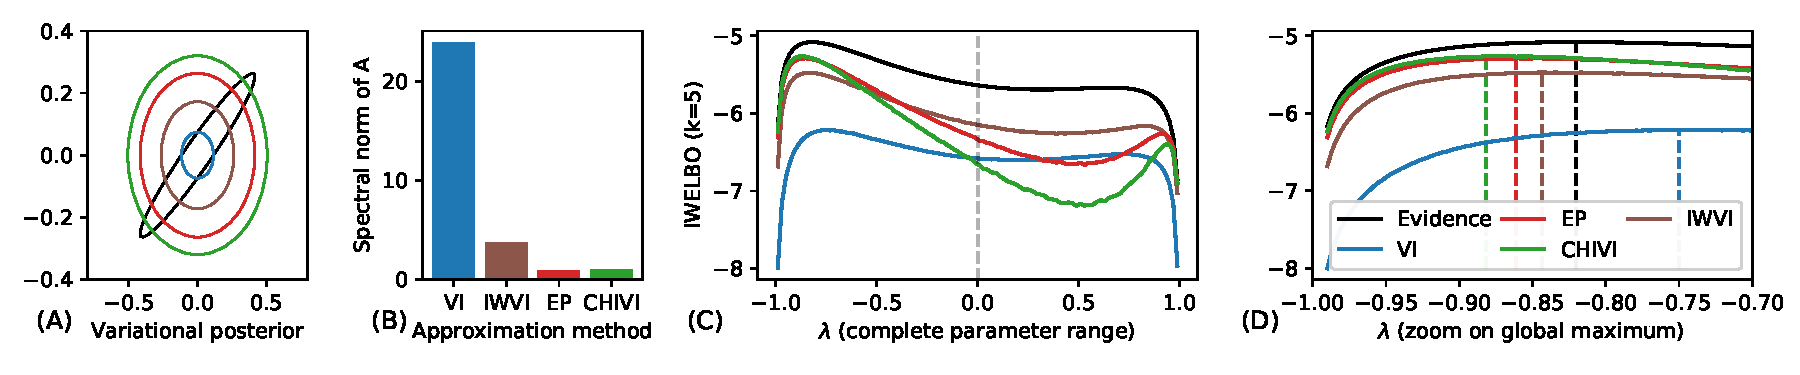
\includegraphics[width=\linewidth]{figures/theoryfull.pdf}
    \caption[Variational Bayes for the bivariate pPCA example.]{Variational Bayes for the bivariate pPCA example. (A) Gaussian mean-field approximations to the posterior (same legend for all the figures) (B) Corresponding values of $\norm{A}_2$ (C) IWELBO ($k=5$) as a function of $\lambda$, with proposals estimated for $\lambda=0$ and other model parameters fixed to their true values (D) Specific zoom around the global maximum.}
    \label{fig:norm_A}
    \vspace{-0.3cm}
\end{figure}

As a consequence of this result, we can characterize the behavior of several variational inference procedures such as EP, CHIVI, IWVI, and VI. We provide this analysis for a bivariate Gaussian example in which all the quantities of interest can be visualized (full derivations in Appendix~\ref{app:biv_gauss}).
Figure~\ref{fig:norm_A}A shows that the VI underestimates the variance while other frameworks provide good coverage of the posterior. As expected, $\norm{A}_2$ is significantly smaller for EP and CHIVI than for VI (Figure~\ref{fig:norm_A}B). 


\subsection{Model selection}
In the VAE framework, the parameter of the model must also be learned. For a fixed variational distribution, variational Bayes (VB) selects the model that maximizes the ELBO or the IWELBO. Each approximate posterior inference method proposes a different lower bound. Even though all these lower bounds becomes tight (equal to the evidence) with a infinite number of particles, the different proposal distribution might not perform equally for model selection because a finite number of particles is used in practice. Moreover, because the optimal IS proposal depends on the target function~\cite{mcbook}, a good proposal for model learning may not be desirable for decision-making and vice versa. 

We can further refine this statement in the regime with few particles. VB estimates of the model parameters are expected to be biased towards the regions where the variational bound is tighter~\cite{Turner2011}. For $k=1$, the tightness of the ELBO is measured by the reverse KL divergence:
\begin{align}
\label{eq:model_selection}
    \kl{q_\phi}{p_\theta} = \frac{1}{2}\left[\textrm{Tr}\left[\Sigma(\theta)^{-1}D(x)\right] + \log \det{\Sigma(\theta)}\right] + C,
\end{align}
where $C$ is constant with respect to $\theta$. Interestingly, because $\kl{p_\theta}{q_\phi}$ is linear in $D(x)$, a higher variance $D(x)$ in Eq.~\eqref{eq:model_selection} induces a higher sensitivity of variational Bayes in parameter space. For $k=5$, no closed-form solution is available so we proceed to numerical experiments on the bivariate pPCA example. In this setting, the approximate posteriors are fit for an initial value of the parameter $\lambda = 0$ (the real value is $\lambda=0.82$) with all other parameters set to their true value. EP and CHIVI exhibit in Figure~\ref{fig:norm_A}C a higher sensitivity than VI and IWVI, similarly to the case $k=1$. This sensitivity translates into higher bias for selection of $\lambda$ (Figure~\ref{fig:norm_A}D). These results suggest that lower variance proposals may be more suitable for model learning than for decision-making, providing yet another motivation for using different proposals for each task.
